\documentclass{article}
\usepackage[utf8]{inputenc}

\title{Climatronic 3000}
\author{Ian Israel García Vázquez | David Hernández Uriostegui}
\date{Octubre 2020}

\usepackage{natbib}
\usepackage{graphicx}
\graphicspath{ {images/} }
\usepackage{listings}

\begin{document}

\maketitle


\section{Definicíon del problema}
El actual AICM necesita un sistema con monitoreo constante que muestra a su gran cantidad de pasajeros el clima de los diversos destinos, asi mismo necesita que el programa solo requiera de iniciarlo y su funcionamiento no dependa de la operación de nadie; los datos requeridos a mostrar son :
    \begin{itemize}
        \item Ciudad (Origen y/o Destino)
        \item Temperatura Máxima y mínima
        \item Humedad
    \end{itemize}
    
\section{Ańalisis del problema}
Dicho problema es claro de requerir un sistema  que procese dichos datos, dichos datos requieren ser solicitados a un servidor cuyos datos esten actualizados; requerirá de algun tipo de funcionamiento con hilos para procesar en paralelo varios aeropuertos.\newline
Por lo tanto debemos encontrar API y herramientos que nos permitan desarrollar este proyecto de la manera más eficiente posible y sin violar el paradigma de Programación Orientada a Objetos, es decir leer las bases de datos y obtener información de la API, lo más eficiente posible sabiendo que contamos con ciertas restricciones .\newline
También debemos considerar todos los errores que puedan surgir ya sea al leer la base de datos o/y los errores que pueda surgir al usar el API
La salida deberá mostrar los datos de forma estética, buena visualización y deberá permitir a cualquier usuario leerlos desde alguna pantalla.

\section{Seleccíon de la mejor alternativa}
Puesto el reto de dicha manera, ha de requerirse un lenguaje de programación con sintáxis sencilla, fácil de leer y escribir, siendo este el menor de los problemas, se requiere un lenguaje que le sea sencillo procesar datos en paralelo, seguro, robusto y fácil de actualizar, asimismo se necesitan de web services que podrán dotarnos de la información, y de igual manera, un paradigma que permitiría modelar este problema de forma sencilla es el Orientado a Objetos;
para ello hemos de seleccionar Python como nuestro lenguaje de programación, su sencilla sintaxis y la gran comunidad que le respaldo ha de proveernos de bastantes herramientas para facilitar el desarrollo del programa, sumada su versatilidad multiparadigma, creemos que puede ser uno de los mejores lenguajes para utilizar y mantener.\\
Como webservice leímos y estudiamos una variada cantidad de opciones, pero hemos de decir que OpenWeatherMap ha terminado por convencernos gracias a su nulo costo, hemos de mencionar que existirán algunas bibliotecas que hemos añadido pues facilitarán el manejo, procesamiento o salida de los datos, pero no habrá de que preocuparse pues serán documentadas en cada sección donde habrán de ser requeridas.
\subsection{ Acerca de los entornos de desarrollo empleados}
        Gracias a la gran versatilidad de Linux, hemos optado por utilizarlo como nuestro sistema operativo modelo; asimismo
        utilizamos editores de Texto de uso común, tales como:\\
        \begin{itemize}
            \item Sublime Text:\\
            Con algunos ajustes propios, y una pantalla compartida a la terminal de linux, es sumamente sencillo utilizarlo, aunado a la ventaja de avisos y autoidentación bajo la personalización otorgada a través de los plugins correspondientes a Python.
            \item Vim:
            Su versatilidad, robustez y confianza a lo largo de los años permite tener una muy completa experiencia de desarrollo, aunado a la terminal de linux, y su permantente presencia para visualizar los errores
            
        \end{itemize}
        
\section{Mantenimiento}
Este programa habrá de requerir ligeros cambios conforme el tiempo vaya continue, y se vayan desarrollando más y mejores tecnologías, ya que posiblemente entre sus nuevas necesidades sea agregar nuevos destinos, y disminuir la complejidad, a pesar de que tenemos claramente una excelente complejidad .\textbf{\textit{O(n)}} gracias al proceso de multithreading, aunque sin este mismo seguiría siendo lineal, pero en tardaría más en realizar las peticiones.
\section{Visualización de mejora a futuro}
Claramente una de las mejoras que podrán ayudar al programa en un futuro próximo es la creación de una interfaz gráfica bastante estética, cuyo objetivo no es más que hacer atractiva la salida de los datos y facilite su lectura. Sumado a ello la mejora de la complejidad para la obtención de datos la creemos posible a pesar de su muy eficiente complejidad de orden lineal. Aunque podríamos tener un mejor diseño y mejorar el manejo de peticiones mediante funciones asincronas y teniendo una API para poder obtener los códigos IATA de una ciudad, y de esta forma hacer el proyecto más reutilizable. Así mismo podríamos hacer este proyecto una Web App de tal manera que tengamos el proyecto montado en un servidor y tal vez implementarlo en un lenguaje de programación con mejor funcionalidad para servicios como JavaScript.

\section{Costos}
Es imperativo mencionar el hecho de que este proyecto ha sido realizado utilizando 125 hrs para desarrollar código de alta calidad, documentación y pruebas unitarias de desarrollo, generando 14 versiones anteriores útiles. Sumado a ello, la valoración del tiempo, el desarrollo propio del programa y todo lo que involucra, aunado al hecho de que el plan de adquisición de este sistema contempla, el mantenimiento y las mejoras a futuro, puede contratarse a través de los siguientes planes:\\

\begin{enumerate}
    \item Contratación del sistema por un año, incluye:\\
    24hrs de asistencia en nuestra Línea de ayuda, mejoras y mantemiento mensual + 1 mes de prueba: $\$ 153,000mxn + $ IVA 
    \item Contratación a 6 meses, incluye:\\
   Asistencia 24 hrs al día en nuestra línea de ayuda, mantenimiento y mejoras mensualmente +   15 días de prueba: $ \$81,000mxn $ + IVA  
   \item Contratación a 1 mes, incluye:\\
   Asistencia 24 hrs al día en nuestra línea de ayuda, mantenimiento de acuerdo a la versión general: $\$28,000 mxn$ + IVA
   
    
\end{enumerate}
Según los actuales márgenes de salarios, contratar a un programador de planta representa un salario de \$20,000 mxn promedio/mes
a lo cual podrán ver, contratar por un año el programa generará apenas una inversión por \$27,000 mxn bimestralmente, es decir los costos se reducen a más de la mitad, sumado al beneficio de un programa diseñado en las manos de la experiencia.

\section{Documentación}
    \subsection{Voz.py}
        \begin{itemize}
            \item
            \begin{lstlistings}
            Builder \textit{\textbf{\_\_init\_\_}(self)} llamado como Voz() - genera una instancia de la clase voz
            
            \end{lstlistings}
            
           \textbf{Métodos}
            \item \textit{\textbf{say}(self, word)}  - A través de una voz cargada, genera un file.mp3 y es reproducido tras ser generado, solo puede ser instanciado desde un objeto Voz
            
            \item \textit{\textbf{say\_slow}(self, word)} - Menciona de forma lenta a través de un archivo mp3 generado.Solo puede ser instanciado desde un objeto Voz
            
            \item \textit{\textbf{save\_audio}(self)} - Genera un audio repitiendo lo insertado en la string y es resguardado en resources/ como saved.mp3. Solo puede ser instanciado desde un objeto Voz.
            
            \item \textit{\textbf{into\_start}(self)} - Reproduce un .mp3 ubicado en la carpeta resources/tones llamado announcement.mp3. Solo puede ser instanciado desde un objeto Voz.
            
            \item \textit{\textbf{greet}(self)} - Saluda de acuerdo a la hora del día y con datos escritos en resources/greeting/greeting\_afternoon.txt y
            resources/greeting/greeting\_morning.txt, selecciona un saludo al azar.
        \end{itemize}
    \subsection{Net.py}
        \begin{itemize}
            \item Builder \textit{\textbf{\_\_init\_\_}(self)}, genera una instacnia de tipo Net\\
            \textbf{Métodos}
            \item \textit{\textbf{test}(self)} - Regresa verdadero sí se encuentra conectado a internet, falso en caso contrario. 
        \end{itemize}
    \subsection{City.py}
        \begin{itemize}
            \item Builder \textit{\textbf{\_\_init\_\_}(self, nombre, temperatura, descripcion, humedad, temp\_max, temp\_min)} - Genera una instancia de tipo City que modela una ciudad en función de los datos requeridos \\\\
            \textbf{Métodos}
            \item \textit{\textbf{set\_hora\_salida}(self, hora\_salida)} - Establece la hora de salida de una ciudad
            \item \textit{\textbf{set\_hora\_llegada}(self, hora\_llegada)} - Establece la hora de llegada de una ciudad
            \item \textit{\textbf{get\_nombre}(self)} - Regresa el nombre de la ciudad
            \item \textit{\textbf{get\_temperatura}(self)} - Regresa la temperatura de la ciudad
            \item \textit{\textbf{get\_descripcion}(self)} - Regresa la descripción del clima de la ciudad
            \item \textit{\textbf{get\_humedad}(self)} - Regresa la humedad de la ciudad
            \item \textit{\textbf{get\_temp\_min}(self)} - Regresa la temperatura mínima de la ciudad
            \item \textit{\textbf{get\_temp\_max}(self)} - Regresa la temperatura máxim de la ciudad
            \item \textit{\textbf{imprime\_ciudad}(self)} - Regresa un diccionario con la información de la ciudad
            \item \textit{\textbf{formato}(self)} - Regresa una cadena con la información en formato para que el asistente de voz lo diga
            \item \textit{\textbf{formato\_salida}(self)} - Regresa una cadena con la informacion lista para ser dicha por la asistente de voz dando información de la hora
            \item \textit{\textbf{\_\_gt\_\_}(self, ciudad)} - Compara una ciudad con otra dado la hora de salida y llegada
            \item \textit{\textbf{\_\_str\_\_}(self)} - Regresa la representación en cadena de una ciudad
            \end{itemize}
        \subsection{AnalizadorDatos.py}
            \begin{itemize}
            \item Builder \textit{\textbf{\_\_init\_\_}(self)} - Genera una instancia de tipo AnalizadorDatos que lo modela un Analizador de datos para procesar los datos de las 2 bases de datos \\\\
            \textbf{Métodos}
            \item \textit{\textbf{get\_ciudades}(self)} - Regresa un diccionario donde las llaves son el código IATA de las ciudades del dataset1.cvs y las valorws son el nombre de la ciudad que le corresponde al código IATA
            \item \textit{\textbf{get\_cache}(self)} - Regresa un diccionario donde las llaves el nombre de las ciudades que ya han sido procesadas mediante un request y los valores son la instacia de tipo City correspondiente al nombre de la ciudad
            \item \textit{\textbf{get\_counter}(self)} - Regresa el contador de peticiones totales
            \item \textit{\textbf{crea\_ciudad}(self, url, nombre, session)} - Crea una ciudad a partir de un request 
            \item \textit{\textbf{ciudades\_set1}(self)} - Procesa todos los vuelos del dataset1, llegada y destino. Regresa un conjunto de tuplas donde cada tupla es un vuelo 
            \item \textit{\textbf{ciudades\_set2}(self)} - Procesa todos los vuelos del dataset2. Regresa un conjunto con todas las ciudades validas y no validas (muy pocas) del dataset2 
            \item \textit{\textbf{destino\_llegada}(self, ciudad\_origen, ciudad\_destino)} - Regresa una cadena con la información de un vuelo 
            \item \textit{\textbf{verifica\_cacheSet1}(self, api\_adrees, ciudad1, ciudad2, session)} - Verifica si ciudad1 y ciudad están en el cahcé, si no las procesa mediante un request e imprime la información de las ciudades
            \item \textit{\textbf{verifica\_cacheSet2}(self, api\_adrees, s, session)} - Verifica si \textit{s} está en el caché, si no la procesa mediante un request e imprime la información de las ciudad correspondiente a \textit{s}
            \item \textit{\textbf{show\_dataSet1}(self)} - Procesa los datos del dataset1 mediante Multithreading y nos regresa la información deseada
            \item \textit{\textbf{show\_dataSet2}(self)} - Procesa los datos del dataset2 mediante Multithreading y nos regresa la información deseada
            \item \textit{\textbf{emergent\_advertisment}(self)} - Función auxliar para relacionar las ciudades por hora de salida y repetir a voz
            \item \textit{\textbf{advertisment}(self, cadena\_formato, formato\_salida)} - Imprime la información de una ciudad  y la repite a voz
        \subsection{Tiempo.py}
            \begin{itemize}
                \item Builder \textit{\textbf{\_\_init\_\_}(self)} - Genera una instancia de tipo Tiempo clase que modela el tiempo dado el año, mes, día y hora \\\\
                \textbf{Métodos}
                 \item \textit{\textbf{get\_local\_date}(self)} - Regresa la fecha local
                 \item \textit{\textbf{get\_lhour}(self)} - Regresa la hora local
                 \item \textit{\textbf{get\_local\_time}(self)} - Regresa el tiempo local (AM) o (PM)
                 \item \textit{\textbf{get\_year}(self)} - Regresa el año actual
                 \item \textit{\textbf{get\_month}(self)} - Regresa el mes local
                 \item \textit{\textbf{get\_day}(self)} - Regresa el día local
                 \item \textit{\textbf{get\_sun}(self)} - Regresa el tiempo local (AM) o (PM)
                 \item \textit{\textbf{convert\_into\_hour}(self, hora\_string)} - Regresa una hora convertida en fecha
            \end{itemize}
        
        \section{Descripción del Sistema}
            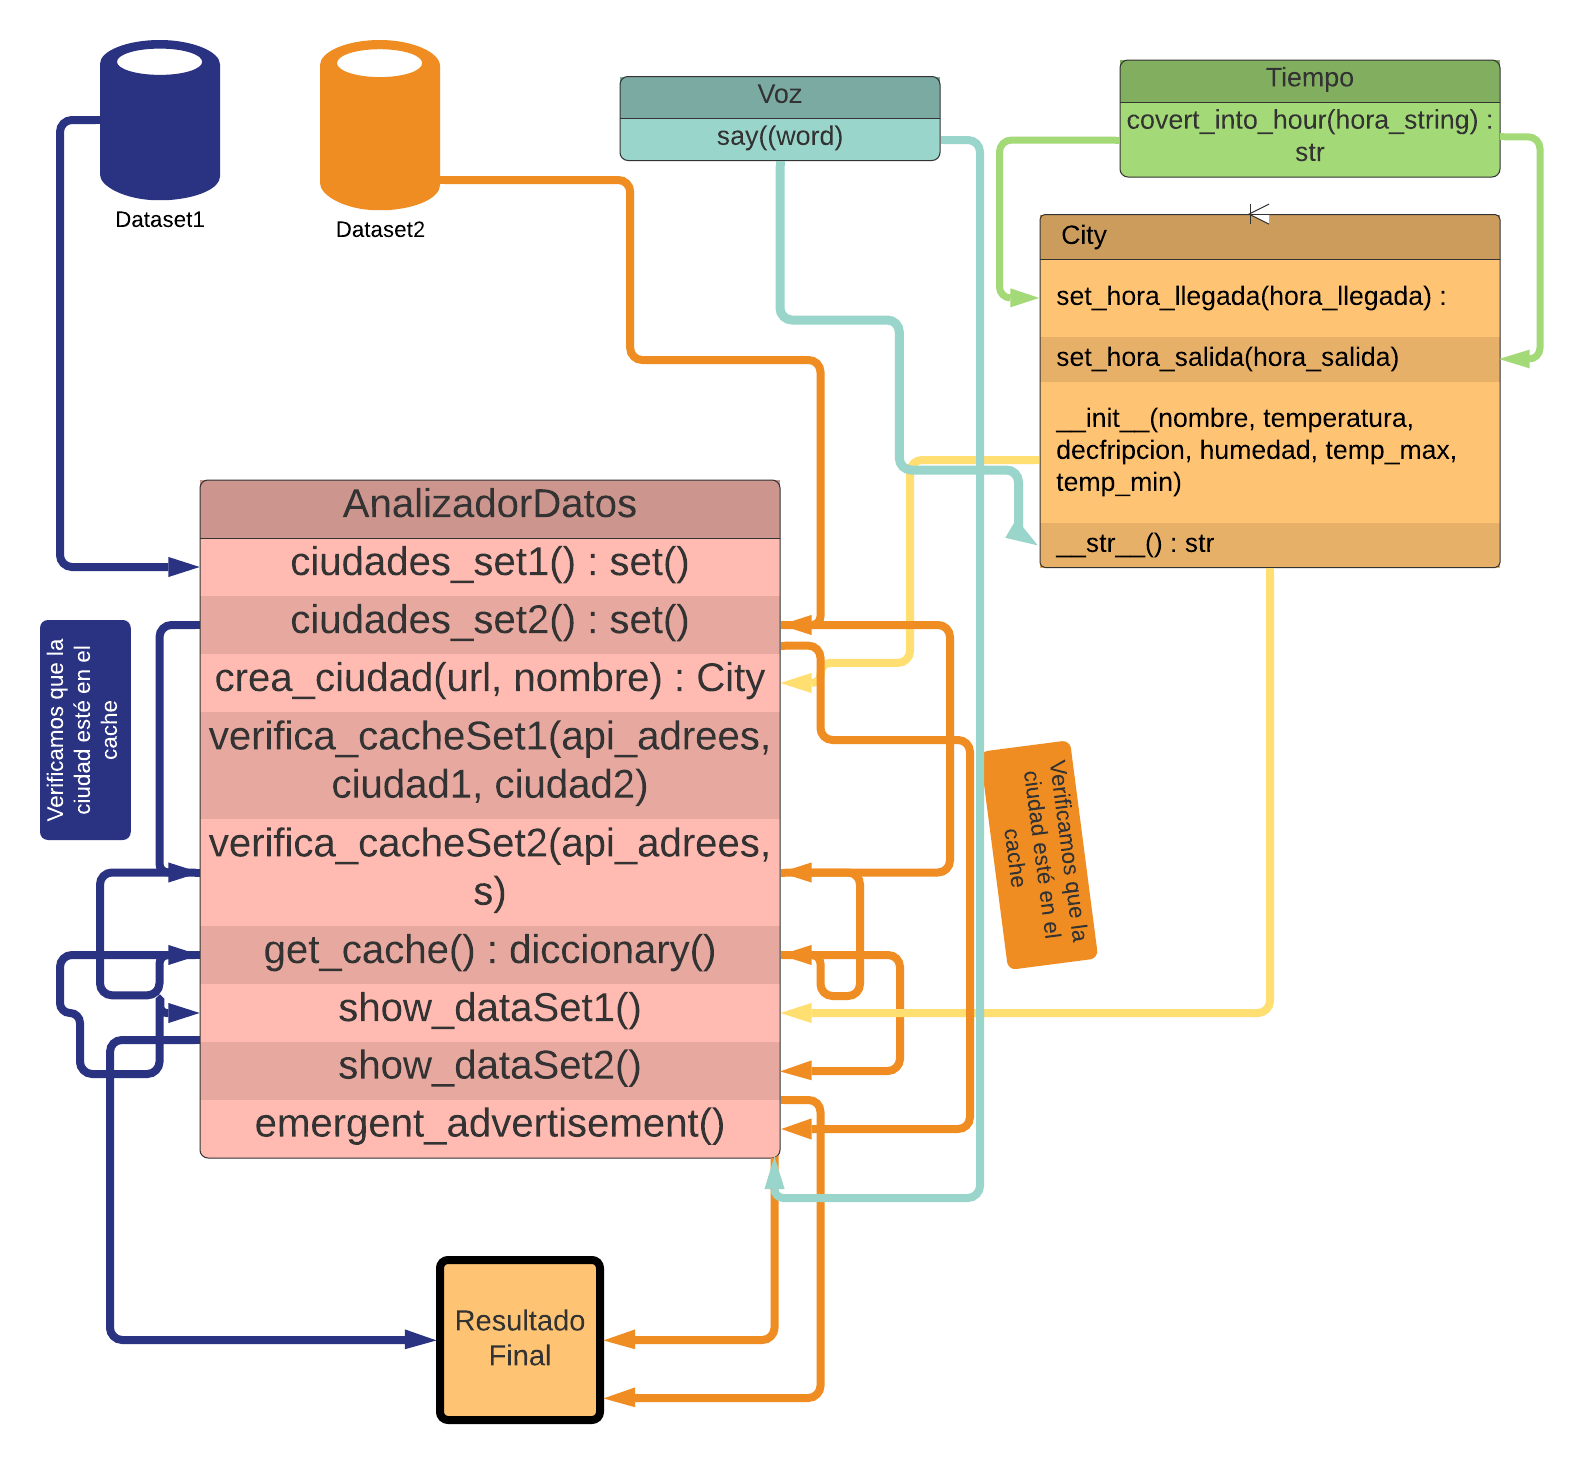
\includegraphics[scale=0.2]{flujo} \\
            Lo que se trató en este proyecto fue realizar las peticiones necesarias en el menor tiempo posible, el tiempo real para el total de peticiones tomando el limit rate de la API es de 16 minutos aproximadamente.
            Al final el proyecto en el mejor de los casos tarda 3.5 - 4 minutos con un buen internet, con un internet que tiende a tener una velocidad más lenta entre 4 - 5 minutos, esto gracias a la herramienta ThreadPoolExecutor que nos proporciona la bibloteca concurrent.futures de Python.
            El proceso es el siguiente:
            \begin{itemize}
                \item \textbf{Procesamos las entradas: } Para las entradas se nos proporciona 2 bases de datos diferentes.
                \begin{itemize}
                    \item \textbf{Dataset1: } Lo que hacemos con la bibloteca de pandas es sólo leer las columnas de Origen y Destino para crear un conjunto de tuplas, donde cada tupla representa un vuelo, de esta forma nos aseguramos de tener todos los vuelos que se producen en el dataset1.
                    \item \textbf{Dataset2: } Lo que hacemos con la bibloteca de pandas es sólo leer la columna de Ciudades para crear un conjunto de strings, donde cada string representa una ciudad, aunque el conjuno puede contener ciudades invalidas.
                \end{itemize}
                \item \textbf{Verificamos Caché: } Tenemos un caché para así evitar hacer más peticiones de las necesarias, el caché.
                El siguiente paso que hacemos es:
                \begin{itemize}
                    \item \textbf{Para el DataSet1: } Pasamos a procesar la información que obtuvimos anteriormente, es decir, el conjunto que obtuvimos.
                    Por cada tupla en el conjunto hacemos lo siguiente: Obtenemos el nombre de las ciudades a partir de código IATA ya que en el Dataset1 las ciudades viene dados en códigos IATA, después verificamos si las 2 ciudades en el caché para así evitar hacer peticiones inncesarias.
                    \begin{itemize}
                        \item \textbf{Caso 1: Las 2 ciudades están en el caché: } En este caso sólo obtenemos la información del caché de las 2 ciudades
                        \item \textbf{Caso 2: La ciudad de origen está en el cahcé, pero la de destino no: } En este caso obtenemos la información de la ciudad de origen del caché, mientrás que para la de destino hacemos un request a la API para obtener la información de la ciudad
                        \item \textbf{Caso 3: La ciudad de destino está en el cahcé, pero la de origen no: } Este caso es analogo al anterior, sólo que se invierte destino y origen
                        \item \textbf{Caso 4: Ninguna de las ciudades están en el caché } En este caso no nos queda de otra, más hacer 2 request a la API para obtener la información de las 2 ciudades
                    \end{itemize}
                    Después de haber hecho este proceso imprimimos la información de las 2 ciudades cómo si fuera un vuelo
                    \item \textbf{Para el DataSet2: } Es el mismo proceso, la única diferencia es que el conjunto que vamos a procesar es de strings, son vuelos que salen solamente de la Ciudad de México, entonces aqui sólo tomamos en cuanta el caso en que la ciudad ya esté en el caché o no.
                \end{itemize}
                \item \textbf{Usamos el ThreadPoolExecutor } Aqui lo que hacemos es usar una excelente función que nos proporciona esta herramienta. Lo que hace esto es que podemos pasarla al ThreadPoolExecutor una cantidad arbitraria de hilos para que hagan un trabajo. Mandamos a llamar a las funciones que hacen el procesamiento de las ciudades y las pasamos al ThreadPoolExecutor. Para procesar aproximadamente en 3-10 segundos el Dataset1 usamos 15 hilos y para el Dataset2 usamps 10 esto debido a evitar un baneo de la API. Asi podemos procesar toda la información de manera más rápida, aunque como se mencionó antes, investigamos un poco más y esto podría llegar a ser más eficiente usando funciones asincronas, sólo que por el tiempo ya no tuvimos tiempo de implemntarlo
                \item \textbf{Asistente de voz } Finalmente como pequeño detalle añadimos un auxiliar de voz que va avisando de los vuelos, para modelar un poco un aeropuerto y de esta manera sea más interactivo para el usuario.
                
            \end{itemize}
        \end{itemize}
        \section{Conclusión}
            Como conclusión este proyecto fue bastante divertido e interesante de hacer, nos permitió ver la diferencia de usar un diferente lenguaje de programación, así como dos cosas que podemos llegar a hacer en un ambito laborar (Ciencia de datos y Web Development), también nos permitió saber que para elaborar un pequeño por lo más pequeño que sea, hay saber analizar el problema y saber diseñar un programa robuesto que sea lo menos propenso a errores, ya que como se dijo en clase: \textbf{Ningún programador está excento de tener algún bug en su código y esto lo vemos día con día.}
            
        \end{itemize}
        
    
    
        
           


\end{document}
